% =============================================================
%  Series compensation
%  Figures copied from presentation/design/ac-transmission/fig/
%  (sc_*.pdf), generated by that folder's series_compensation_figures.py
%  from the exact two-port equations with the bank cascaded as a
%  series element.  Worked line: the 500 kV reference line of Section 6.
% =============================================================
\subsection{Series Compensation}
\label{sec:series-compensation}

\subsubsection{Principle}
\label{sec:sc-principle}

A capacitor bank in series with the line cancels part of its inductive
reactance. The degree of compensation is defined against the total series
reactance,
\begin{equation}
  k = \frac{X_C}{X_L},
  \qquad X_L = \omega \cdot L' \cdot l,
  \qquad X_{eff} = \left(1-k\right) \cdot X_L
  \label{eq:sc-k}
\end{equation}
so that the lossless transfer becomes
\begin{equation}
  P = \frac{U^2}{\left(1-k\right) \cdot X_L} \cdot \sin\delta
  \label{eq:sc-power}
\end{equation}
with $\left|U_S\right| = \left|U_R\right| = U$. The line behaves as though
it were shorter: for a given transfer the angle falls and the stability
margin of Section~\ref{sec:angular-stability} rises.

Two properties distinguish it from shunt compensation. The voltage rise
$I \cdot X_C$ across the bank scales with the current, so the compensation
is self-regulating: it appears when it is needed and not at light load. And
it acts on the series branch, which is why it addresses the angular limit
and barely moves the voltage limit of case~(a) in
Section~\ref{sec:limits-compensation}.

The practical range is $k \approx 0.25 \ldots 0.70$. Above that,
sub-synchronous resonance, distance-protection behaviour and bank cost
dominate the choice.

In the two-port model the bank is cascaded as a series element at the point
where it is installed,
\begin{equation}
  \begin{bmatrix} 1 & -j \cdot X_C \\ 0 & 1 \end{bmatrix}
  \label{eq:sc-twoport}
\end{equation}
between the two half-lines for a midpoint bank, which is the arrangement
used throughout this section.

\subsubsection{Single-line arrangement}
\label{sec:sc-sld}

A series bank is not only capacitors. The platform sits at line potential
and carries the full fault current until it is bypassed, so each phase
carries a metal-oxide varistor across the bank to limit the capacitor
voltage under fault current, a bypass breaker with a damping reactor to take
over when the varistor reaches its energy limit, and disconnectors to
isolate the platform. A bypass disconnector keeps the line in service with
the bank out, at $k = 0$. Figure~\ref{fig:sc-sld} shows the arrangement for
one phase, with the bank at the midpoint of the line.

\begin{figure}[!ht]
  \centering
  \begin{tikzpicture}[x=1.07mm, y=1.07mm,
      wire/.style={draw=atFg, line width=0.35mm, line cap=round, line join=round},
      hair/.style={draw=atFg, line width=0.22mm, line cap=round, line join=round},
      bus/.style={draw=atFg, line width=0.9mm, line cap=butt},
      lbl/.style={font=\footnotesize, atFg},
      sub/.style={font=\scriptsize, atFgMuted},
      dot/.style={fill=atFg, circle, inner sep=0pt, minimum size=1.1mm}]
    % buses and line
    \draw[bus] (0,-8) -- (0,8);     \node[lbl,above] at (0,8.5) {S};
    \draw[bus] (120,-8) -- (120,8); \node[lbl,above] at (120,8.5) {R};
    \draw[wire] (0,0) -- (30,0);
    \draw[wire] (90,0) -- (120,0);
    \node[sub] at (15,3.2) {$l/2$};
    \node[sub] at (105,3.2) {$l/2$};
    % line disconnectors into the platform
    \draw[wire] (30,0) -- (33,0);
    \draw[wire] (33,0) -- (38.5,3.5);
    \draw[wire] (39,0) -- (42,0);
    \node[sub,above] at (36,4) {DS1};
    \draw[wire] (78,0) -- (81,0);
    \draw[wire] (81,0) -- (86.5,3.5);
    \draw[wire] (87,0) -- (90,0);
    \node[sub,above] at (84,4) {DS2};
    % main branch: series capacitor
    \node[dot] at (42,0) {};  \node[dot] at (78,0) {};
    \draw[wire] (42,0) -- (57,0);
    \draw[wire] (57,-4) -- (57,4);  \draw[wire] (60,-4) -- (60,4);
    \draw[wire] (60,0) -- (78,0);
    \node[lbl,above] at (58.5,4.8) {$C$\quad{\scriptsize\color{atFgMuted}$X_C = k \cdot X_L$}};
    % MOV branch
    \draw[wire] (42,0) -- (42,-10) -- (54,-10);
    \draw[wire] (54,-13) rectangle (66,-7);
    \draw[hair] (55,-12) -- (65,-8);
    \draw[wire] (66,-10) -- (78,-10) -- (78,0);
    \node[sub,below] at (60,-13.3) {MOV};
    % damping reactor and bypass breaker
    \draw[wire] (42,-10) -- (42,-20) -- (50,-20);
    \draw[wire] (50,-22) rectangle (58,-18);
    \draw[wire] (58,-20) -- (63,-20);
    \draw[wire] (63,-22) -- (67,-18);  \draw[wire] (63,-18) -- (67,-22);
    \draw[wire] (67,-20) -- (78,-20) -- (78,-10);
    \node[sub,below] at (54,-22.3) {$L_d$};
    \node[sub,below] at (65,-22.3) {bypass CB};
    % bypass disconnector around the whole bank
    \draw[wire] (33,0) -- (33,-33) -- (55,-33);
    \draw[wire] (55,-33) -- (60.5,-29.5);
    \draw[wire] (61,-33) -- (87,-33) -- (87,0);
    \node[sub,below] at (58,-34) {bypass DS};
    % platform outline
    \draw[atFgMuted, line width=0.4pt, densely dashed] (39,-27.5) rectangle (81,12.5);
    \node[sub,anchor=south east] at (81,12.8) {capacitor platform, line potential};
    % current arrow
    \draw[-{Stealth[length=2mm]}, atFgMuted] (8,-3.5) -- (22,-3.5)
      node[midway,below,sub] {$I$};
  \end{tikzpicture}
  \caption{Single-line diagram of a midpoint series bank, one phase.
           Symbols to IEC 60617~[18]}
  \label{fig:sc-sld}
\end{figure}

The varistor limits the capacitor voltage under fault current and the bypass
breaker with its damping reactor $L_d$ takes over at the varistor energy
limit. DS1 and DS2 isolate the platform; the bypass disconnector keeps the
line in service with the bank out.

\subsubsection{Effect on the power-angle curve}
\label{sec:sc-power-angle}

Figure~\ref{fig:sc-power-angle} shows the power-angle curves of the 500\,kV
reference line for a midpoint bank at several degrees of compensation, and
Table~\ref{tab:sc-power-angle} the resulting maxima.

\begin{figure}[!ht]
  \centering
  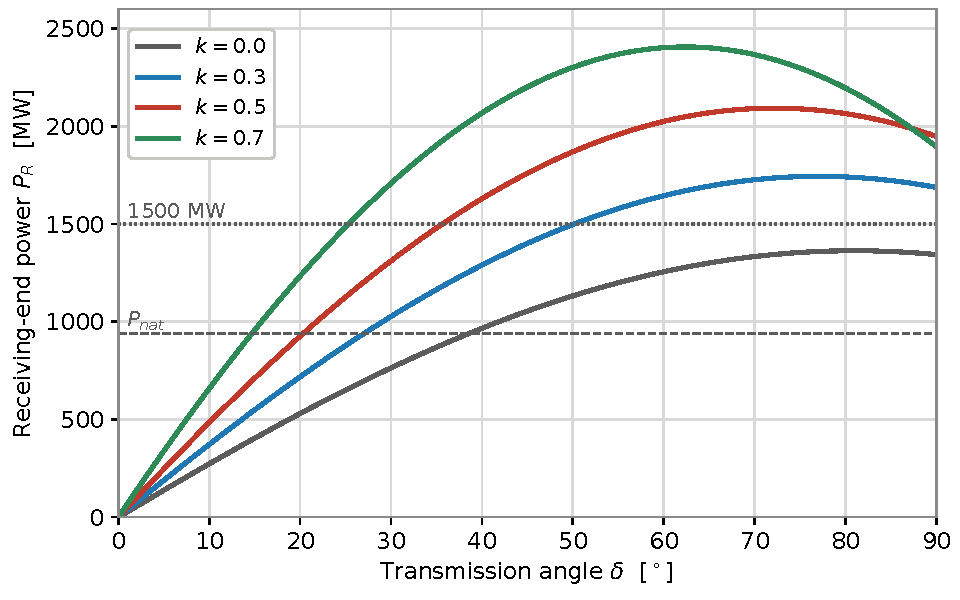
\includegraphics[width=0.74\linewidth]{figures/ac/sc_power_angle.pdf}
  \caption{Power-angle curves of the reference line with a midpoint series
           bank, both terminals at 1.0\,p.u.}
  \label{fig:sc-power-angle}
\end{figure}

\begin{table}[!ht]
  \centering
  \begin{tabular}{@{}c r r r@{}}
    \toprule
    \textbf{$k$} & \multicolumn{1}{c}{\textbf{$X_C$}}
      & \multicolumn{1}{c}{\textbf{$P_{max}$}}
      & \multicolumn{1}{c}{\textbf{$\delta$ at 1500\,MW}} \\
    & \multicolumn{1}{c}{$\Omega$} & \multicolumn{1}{c}{MW}
      & \multicolumn{1}{c}{$^\circ$} \\
    \midrule
    0   & 0     & 1363 & --- \\
    0.3 & 48.7  & 1744 & 50.1 \\
    0.5 & 81.2  & 2093 & 35.7 \\
    0.7 & 113.7 & 2407 & 25.3 \\
    \bottomrule
  \end{tabular}
  \caption{Midpoint bank on the 300\,mi reference line, exact two-port}
  \label{tab:sc-power-angle}
\end{table}

Uncompensated, 1500\,MW --- $1.6 \cdot P_{nat}$ --- cannot be carried at
all; at $k = 0.5$ it is carried at $36^\circ$. The maximum also moves to
smaller angles as $k$ grows, which is the electrical shortening of the line
expressed on the curve. The lossless form
$U^2 / \left(\left(1-k\right) \cdot X_L\right)$ would give 1540\,MW
uncompensated and 3080\,MW at $k = 0.5$; at this length $R = 27.5\,\Omega$
and the line charging are not negligible, which is why the exact two-port is
used.

\subsubsection{Voltage profile at heavy load}
\label{sec:sc-voltage}

Delivering 900\,MW at $\cos\varphi = 0.95$ lagging with the receiving end
held at 1.0\,p.u., the uncompensated line requires a sending-end voltage of
1.217\,p.u., far outside any operating band. The midpoint bank lifts the
voltage by $I \cdot X_C$ in the direction of power flow, and the sending end
falls to 1.157, 1.127 and 1.107\,p.u.\ for $k = 0.3$, 0.5 and 0.7,
Figure~\ref{fig:sc-voltage}.

\begin{figure}[!ht]
  \centering
  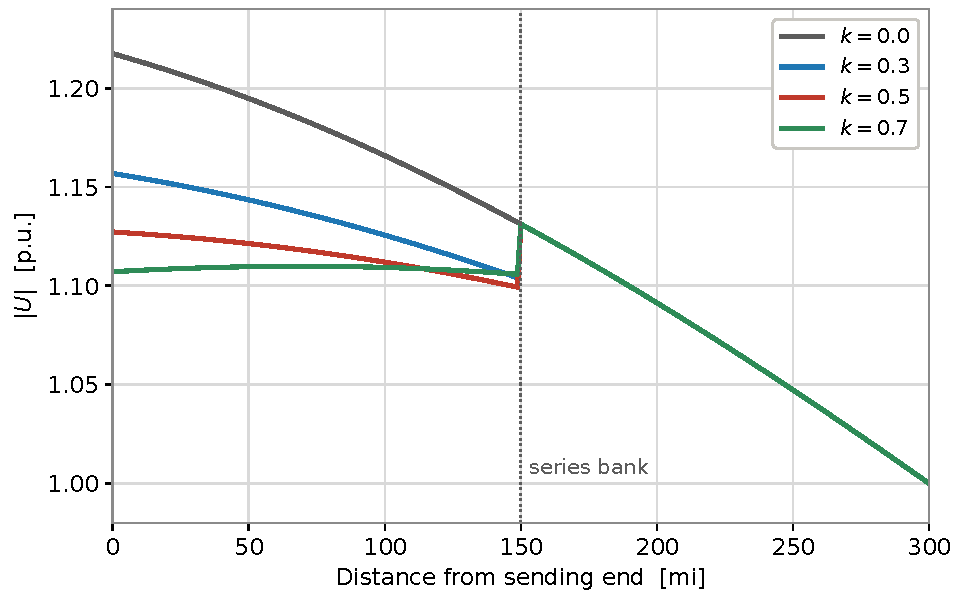
\includegraphics[width=0.74\linewidth]{figures/ac/sc_voltage_profile.pdf}
  \caption{Voltage profile at heavy load with a midpoint series bank}
  \label{fig:sc-voltage}
\end{figure}

The receiving half of the line is unchanged, because the bank acts only on
what is upstream of it. That is why end-of-line banks and split banks are
also used where the voltage profile rather than the angle is the problem.

\FloatBarrier

\subsubsection{Bank rating and protection}
\label{sec:sc-rating}

The bank is rated for the planned continuous line current, not for the
conductor thermal limit:
\begin{equation}
  U_C = I_{rated} \cdot X_C
  \qquad
  Q_C = 3 \cdot I_{rated}^{2} \cdot X_C
  \label{eq:sc-rating}
\end{equation}
Table~\ref{tab:sc-rating} gives the resulting bank for the reference line at
$k = 0.5$.

\begin{table}[!ht]
  \centering
  \begin{tabular}{@{}l l r@{}}
    \toprule
    \textbf{Quantity} & & \multicolumn{1}{c}{\textbf{Value}} \\
    \midrule
    $k$ & & 0.5 \\
    $X_C$ & $\Omega$ & 81.2 \\
    $C$ per phase & \textmu F & 32.7 \\
    $I_{rated}$ & A & 2000 \\
    \midrule
    $U_C$ per phase & kV & 162 \\
    $Q_C$ three-phase & MVAr & 974 \\
    MOV level ($2.3 \cdot U_C$) & kV & 373 \\
    \bottomrule
  \end{tabular}
  \caption{Midpoint bank rating on the reference line at $k = 0.5$}
  \label{tab:sc-rating}
\end{table}

$I_{rated}$ is taken as about $1.15 \cdot$ the current at 1500\,MW and
500\,kV. The fault-current voltage is limited by the metal-oxide varistor at
a protective level of $2.0 \ldots 2.5 \cdot U_C$, with the bypass breaker
and damping circuit behind it. Emergency ratings --- typically 30\,min and
10\,s --- are specified separately from the continuous rating.

\subsubsection{Sub-synchronous resonance}
\label{sec:sc-ssr}

The bank forms a series resonance with the line and source reactances at
\begin{equation}
  f_{er} = f_0 \cdot \sqrt{\frac{X_C}{X_L + X_S}}
  \label{eq:sc-ssr}
\end{equation}
Rotor currents see the complement $f_0 - f_{er}$, which has to stay clear of
the torsional modes of the turbine-generator shaft --- 10 to 45\,Hz for
large steam units. Figure~\ref{fig:sc-ssr} screens the reference line against
the degree of compensation.

\begin{figure}[!ht]
  \centering
  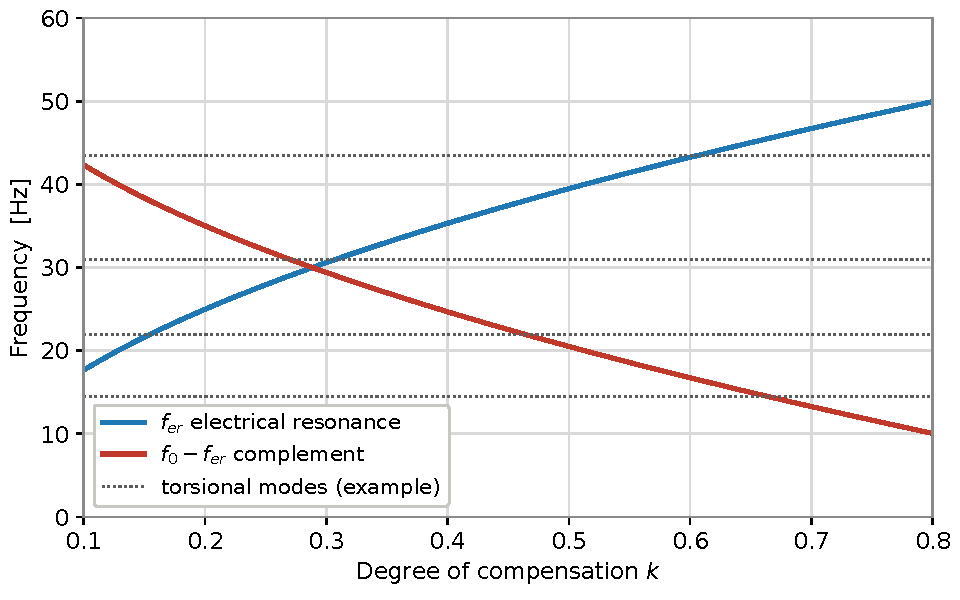
\includegraphics[width=0.72\linewidth]{figures/ac/sc_ssr_screening.pdf}
  \caption{Sub-synchronous resonance screening: electrical resonance and its
           complement against the degree of compensation}
  \label{fig:sc-ssr}
\end{figure}

With $X_S = 25\,\Omega$, which is 15\,\% on 1500\,MVA, a compensation of
$k = 0.5$ gives $f_{er} = 39.5$\,Hz and a complement of 20.5\,Hz --- within
2\,Hz of an illustrative 22\,Hz torsional mode. A hit at screening level
calls for a detailed study or a different $k$; type-3 wind generation adds
sub-synchronous control interaction to the same screening. The torsional
modes used at this stage are illustrative, and real values come from the
generator manufacturer.

\FloatBarrier
